\documentclass[border=0cm]{standalone}
\usepackage{tikz}
\usetikzlibrary{arrows, arrows.meta}
\tikzset{    
    barbarrow/.style={ % style that just defines the arrow tip
        >={Straight Barb[left,length=5pt,width=5pt]},
        thick,
        <->
    },
    blues/.style={
        color=blue
    },
    reds/.style={
        color=red
    }
}
\definecolor{light-gray}{gray}{0.9}

\begin{document}
\begin{tabular}{@{}c@{}}
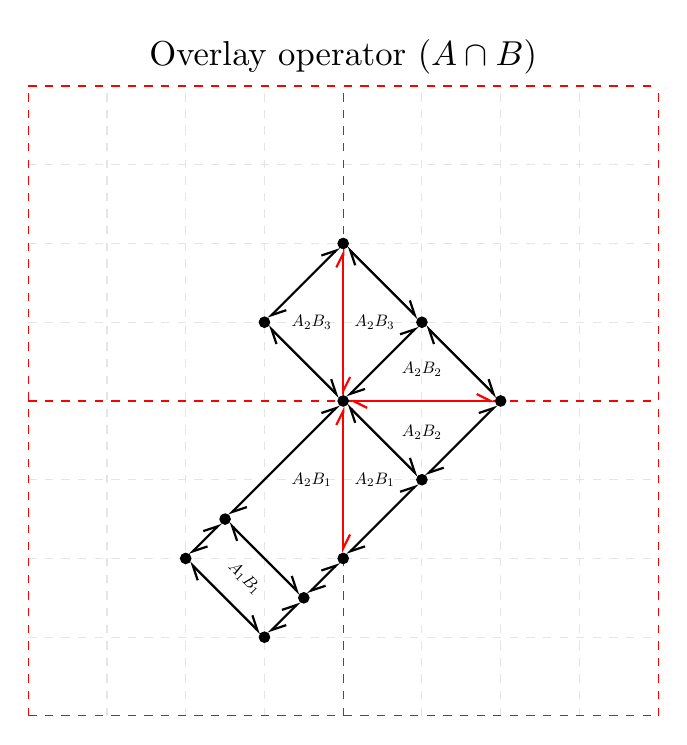
\begin{tikzpicture}
    \tikzstyle{node1}=[draw,scale=0.4,shape=circle,color=black,fill=black]
    \tikzstyle{node2}=[draw,scale=0.4,shape=circle,color=red,fill=red]    
    \draw[color=light-gray, style=dashed] (0,0) grid (8,8);
    \draw[color=red, style=dashed, step=4] (0,0) grid (8,8);
    \node[above, scale=1.25] at (4,8) {Overlay operator ($A \cap B$)};
    \node[node1] (D) at (2,2) {};    
    \node[node1] (G) at (3,1) {};
    \node[node1] (H) at (2.5,2.5) {};
    \node[node1] (I) at (3,5) {};
    \node[node1] (K) at (4,2) {};
    \node[node1] (L) at (4,4) {};    
    \node[node1] (M) at (4,6) {};
    \node[node1] (O) at (5,3) {};
    \node[node1] (P) at (5,5) {};    
    \node[node1] (R) at (6,4) {};    

    \node[node1] (Y) at (3.5,1.5) {};
    
    \node[scale=0.6, rotate=-45] at (2.75,1.75) {$A_1B_1$};
    \node[scale=0.6] at (3.6,3)    {$A_2B_1$};
    \node[scale=0.6] at (4.4,3)    {$A_2B_1$};
    \node[scale=0.6] at (5,4.4)    {$A_2B_2$};
    \node[scale=0.6] at (5,3.6)    {$A_2B_2$};
    \node[scale=0.6] at (3.6,5)    {$A_2B_3$};
    \node[scale=0.6] at (4.4,5)    {$A_2B_3$};
    
    \draw[barbarrow] (G) -- (Y);
    \draw[barbarrow] (Y) -- (K);


    \draw[barbarrow] (D) -- (G);
    \draw[barbarrow] (D) -- (H);
    \draw[barbarrow] (H) -- (L);\draw[barbarrow] (I) -- (L);
    \draw[barbarrow] (I) -- (M);
    %\draw[barbarrow] (G) -- (K);
    \draw[barbarrow] (H) -- (Y);
    \draw[barbarrow] (K) -- (O);\draw[barbarrow] (L) -- (O);
    \draw[barbarrow] (L) -- (P);\draw[barbarrow] (M) -- (P);
    \draw[barbarrow] (O) -- (R);\draw[barbarrow] (P) -- (R);
    
    \draw[barbarrow, color=red] (L) -- (R);
    \draw[barbarrow, color=red] (L) -- (M);
    \draw[barbarrow, color=red] (L) -- (K);

\end{tikzpicture}
\end{tabular}
\end{document}
